% Options for packages loaded elsewhere
\PassOptionsToPackage{unicode}{hyperref}
\PassOptionsToPackage{hyphens}{url}
%
\documentclass[
]{article}
\usepackage{amsmath,amssymb}
\usepackage{iftex}
\ifPDFTeX
  \usepackage[T1]{fontenc}
  \usepackage[utf8]{inputenc}
  \usepackage{textcomp} % provide euro and other symbols
\else % if luatex or xetex
  \usepackage{unicode-math} % this also loads fontspec
  \defaultfontfeatures{Scale=MatchLowercase}
  \defaultfontfeatures[\rmfamily]{Ligatures=TeX,Scale=1}
\fi
\usepackage{lmodern}
\ifPDFTeX\else
  % xetex/luatex font selection
\fi
% Use upquote if available, for straight quotes in verbatim environments
\IfFileExists{upquote.sty}{\usepackage{upquote}}{}
\IfFileExists{microtype.sty}{% use microtype if available
  \usepackage[]{microtype}
  \UseMicrotypeSet[protrusion]{basicmath} % disable protrusion for tt fonts
}{}
\makeatletter
\@ifundefined{KOMAClassName}{% if non-KOMA class
  \IfFileExists{parskip.sty}{%
    \usepackage{parskip}
  }{% else
    \setlength{\parindent}{0pt}
    \setlength{\parskip}{6pt plus 2pt minus 1pt}}
}{% if KOMA class
  \KOMAoptions{parskip=half}}
\makeatother
\usepackage{xcolor}
\usepackage[margin=1in]{geometry}
\usepackage{color}
\usepackage{fancyvrb}
\newcommand{\VerbBar}{|}
\newcommand{\VERB}{\Verb[commandchars=\\\{\}]}
\DefineVerbatimEnvironment{Highlighting}{Verbatim}{commandchars=\\\{\}}
% Add ',fontsize=\small' for more characters per line
\usepackage{framed}
\definecolor{shadecolor}{RGB}{248,248,248}
\newenvironment{Shaded}{\begin{snugshade}}{\end{snugshade}}
\newcommand{\AlertTok}[1]{\textcolor[rgb]{0.94,0.16,0.16}{#1}}
\newcommand{\AnnotationTok}[1]{\textcolor[rgb]{0.56,0.35,0.01}{\textbf{\textit{#1}}}}
\newcommand{\AttributeTok}[1]{\textcolor[rgb]{0.13,0.29,0.53}{#1}}
\newcommand{\BaseNTok}[1]{\textcolor[rgb]{0.00,0.00,0.81}{#1}}
\newcommand{\BuiltInTok}[1]{#1}
\newcommand{\CharTok}[1]{\textcolor[rgb]{0.31,0.60,0.02}{#1}}
\newcommand{\CommentTok}[1]{\textcolor[rgb]{0.56,0.35,0.01}{\textit{#1}}}
\newcommand{\CommentVarTok}[1]{\textcolor[rgb]{0.56,0.35,0.01}{\textbf{\textit{#1}}}}
\newcommand{\ConstantTok}[1]{\textcolor[rgb]{0.56,0.35,0.01}{#1}}
\newcommand{\ControlFlowTok}[1]{\textcolor[rgb]{0.13,0.29,0.53}{\textbf{#1}}}
\newcommand{\DataTypeTok}[1]{\textcolor[rgb]{0.13,0.29,0.53}{#1}}
\newcommand{\DecValTok}[1]{\textcolor[rgb]{0.00,0.00,0.81}{#1}}
\newcommand{\DocumentationTok}[1]{\textcolor[rgb]{0.56,0.35,0.01}{\textbf{\textit{#1}}}}
\newcommand{\ErrorTok}[1]{\textcolor[rgb]{0.64,0.00,0.00}{\textbf{#1}}}
\newcommand{\ExtensionTok}[1]{#1}
\newcommand{\FloatTok}[1]{\textcolor[rgb]{0.00,0.00,0.81}{#1}}
\newcommand{\FunctionTok}[1]{\textcolor[rgb]{0.13,0.29,0.53}{\textbf{#1}}}
\newcommand{\ImportTok}[1]{#1}
\newcommand{\InformationTok}[1]{\textcolor[rgb]{0.56,0.35,0.01}{\textbf{\textit{#1}}}}
\newcommand{\KeywordTok}[1]{\textcolor[rgb]{0.13,0.29,0.53}{\textbf{#1}}}
\newcommand{\NormalTok}[1]{#1}
\newcommand{\OperatorTok}[1]{\textcolor[rgb]{0.81,0.36,0.00}{\textbf{#1}}}
\newcommand{\OtherTok}[1]{\textcolor[rgb]{0.56,0.35,0.01}{#1}}
\newcommand{\PreprocessorTok}[1]{\textcolor[rgb]{0.56,0.35,0.01}{\textit{#1}}}
\newcommand{\RegionMarkerTok}[1]{#1}
\newcommand{\SpecialCharTok}[1]{\textcolor[rgb]{0.81,0.36,0.00}{\textbf{#1}}}
\newcommand{\SpecialStringTok}[1]{\textcolor[rgb]{0.31,0.60,0.02}{#1}}
\newcommand{\StringTok}[1]{\textcolor[rgb]{0.31,0.60,0.02}{#1}}
\newcommand{\VariableTok}[1]{\textcolor[rgb]{0.00,0.00,0.00}{#1}}
\newcommand{\VerbatimStringTok}[1]{\textcolor[rgb]{0.31,0.60,0.02}{#1}}
\newcommand{\WarningTok}[1]{\textcolor[rgb]{0.56,0.35,0.01}{\textbf{\textit{#1}}}}
\usepackage{graphicx}
\makeatletter
\def\maxwidth{\ifdim\Gin@nat@width>\linewidth\linewidth\else\Gin@nat@width\fi}
\def\maxheight{\ifdim\Gin@nat@height>\textheight\textheight\else\Gin@nat@height\fi}
\makeatother
% Scale images if necessary, so that they will not overflow the page
% margins by default, and it is still possible to overwrite the defaults
% using explicit options in \includegraphics[width, height, ...]{}
\setkeys{Gin}{width=\maxwidth,height=\maxheight,keepaspectratio}
% Set default figure placement to htbp
\makeatletter
\def\fps@figure{htbp}
\makeatother
\setlength{\emergencystretch}{3em} % prevent overfull lines
\providecommand{\tightlist}{%
  \setlength{\itemsep}{0pt}\setlength{\parskip}{0pt}}
\setcounter{secnumdepth}{-\maxdimen} % remove section numbering
\ifLuaTeX
  \usepackage{selnolig}  % disable illegal ligatures
\fi
\usepackage{bookmark}
\IfFileExists{xurl.sty}{\usepackage{xurl}}{} % add URL line breaks if available
\urlstyle{same}
\hypersetup{
  hidelinks,
  pdfcreator={LaTeX via pandoc}}

\author{}
\date{\vspace{-2.5em}}

\begin{document}

\begin{Shaded}
\begin{Highlighting}[]
\FunctionTok{library}\NormalTok{(ggplot2)}

\CommentTok{\# Bass model parameters}
\NormalTok{M }\OtherTok{\textless{}{-}} \DecValTok{1000}  \CommentTok{\# Total market potential}
\NormalTok{p }\OtherTok{\textless{}{-}} \FloatTok{0.03}  \CommentTok{\# Coefficient of innovation}
\NormalTok{q }\OtherTok{\textless{}{-}} \FloatTok{0.38}  \CommentTok{\# Coefficient of imitation}

\CommentTok{\# Time range}
\NormalTok{t }\OtherTok{\textless{}{-}} \FunctionTok{seq}\NormalTok{(}\DecValTok{0}\NormalTok{, }\DecValTok{20}\NormalTok{, }\AttributeTok{length.out =} \DecValTok{100}\NormalTok{)  }\CommentTok{\# 20 time periods}
\end{Highlighting}
\end{Shaded}

\begin{Shaded}
\begin{Highlighting}[]
\CommentTok{\# Bass model equation for cumulative adoption}
\NormalTok{bass\_diffusion }\OtherTok{\textless{}{-}} \ControlFlowTok{function}\NormalTok{(t, M, p, q) \{}
\NormalTok{  exp\_term }\OtherTok{\textless{}{-}} \FunctionTok{exp}\NormalTok{(}\SpecialCharTok{{-}}\NormalTok{(p }\SpecialCharTok{+}\NormalTok{ q) }\SpecialCharTok{*}\NormalTok{ t)}
  \FunctionTok{return}\NormalTok{(M }\SpecialCharTok{*}\NormalTok{ (}\DecValTok{1} \SpecialCharTok{{-}}\NormalTok{ exp\_term) }\SpecialCharTok{/}\NormalTok{ (}\DecValTok{1} \SpecialCharTok{+}\NormalTok{ (q }\SpecialCharTok{/}\NormalTok{ p) }\SpecialCharTok{*}\NormalTok{ exp\_term))}
\NormalTok{\}}

\CommentTok{\# Compute adoption over time}
\NormalTok{N\_t }\OtherTok{\textless{}{-}} \FunctionTok{bass\_diffusion}\NormalTok{(t, M, p, q)}

\CommentTok{\# Create a data frame for plotting}
\NormalTok{df }\OtherTok{\textless{}{-}} \FunctionTok{data.frame}\NormalTok{(}\AttributeTok{Time =}\NormalTok{ t, }\AttributeTok{Cumulative\_Adopters =}\NormalTok{ N\_t)}
\NormalTok{df}
\end{Highlighting}
\end{Shaded}

\begin{verbatim}
##           Time Cumulative_Adopters
## 1    0.0000000            0.000000
## 2    0.2020202            6.279002
## 3    0.4040404           13.011474
## 4    0.6060606           20.222704
## 5    0.8080808           27.938184
## 6    1.0101010           36.183397
## 7    1.2121212           44.983560
## 8    1.4141414           54.363336
## 9    1.6161616           64.346508
## 10   1.8181818           74.955611
## 11   2.0202020           86.211535
## 12   2.2222222           98.133090
## 13   2.4242424          110.736544
## 14   2.6262626          124.035135
## 15   2.8282828          138.038581
## 16   3.0303030          152.752567
## 17   3.2323232          168.178259
## 18   3.4343434          184.311826
## 19   3.6363636          201.144012
## 20   3.8383838          218.659749
## 21   4.0404040          236.837854
## 22   4.2424242          255.650808
## 23   4.4444444          275.064642
## 24   4.6464646          295.038943
## 25   4.8484848          315.526988
## 26   5.0505051          336.476015
## 27   5.2525253          357.827644
## 28   5.4545455          379.518423
## 29   5.6565657          401.480515
## 30   5.8585859          423.642498
## 31   6.0606061          445.930268
## 32   6.2626263          468.268013
## 33   6.4646465          490.579238
## 34   6.6666667          512.787809
## 35   6.8686869          534.818993
## 36   7.0707071          556.600444
## 37   7.2727273          578.063135
## 38   7.4747475          599.142190
## 39   7.6767677          619.777605
## 40   7.8787879          639.914845
## 41   8.0808081          659.505299
## 42   8.2828283          678.506594
## 43   8.4848485          696.882777
## 44   8.6868687          714.604358
## 45   8.8888889          731.648227
## 46   9.0909091          747.997468
## 47   9.2929293          763.641079
## 48   9.4949495          778.573608
## 49   9.6969697          792.794735
## 50   9.8989899          806.308811
## 51  10.1010101          819.124368
## 52  10.3030303          831.253618
## 53  10.5050505          842.711953
## 54  10.7070707          853.517451
## 55  10.9090909          863.690411
## 56  11.1111111          873.252908
## 57  11.3131313          882.228382
## 58  11.5151515          890.641263
## 59  11.7171717          898.516631
## 60  11.9191919          905.879915
## 61  12.1212121          912.756630
## 62  12.3232323          919.172145
## 63  12.5252525          925.151498
## 64  12.7272727          930.719222
## 65  12.9292929          935.899222
## 66  13.1313131          940.714664
## 67  13.3333333          945.187893
## 68  13.5353535          949.340375
## 69  13.7373737          953.192650
## 70  13.9393939          956.764305
## 71  14.1414141          960.073966
## 72  14.3434343          963.139291
## 73  14.5454545          965.976983
## 74  14.7474747          968.602798
## 75  14.9494949          971.031578
## 76  15.1515152          973.277269
## 77  15.3535354          975.352955
## 78  15.5555556          977.270896
## 79  15.7575758          979.042556
## 80  15.9595960          980.678647
## 81  16.1616162          982.189164
## 82  16.3636364          983.583419
## 83  16.5656566          984.870087
## 84  16.7676768          986.057234
## 85  16.9696970          987.152358
## 86  17.1717172          988.162423
## 87  17.3737374          989.093890
## 88  17.5757576          989.952752
## 89  17.7777778          990.744565
## 90  17.9797980          991.474473
## 91  18.1818182          992.147242
## 92  18.3838384          992.767279
## 93  18.5858586          993.338665
## 94  18.7878788          993.865169
## 95  18.9898990          994.350278
## 96  19.1919192          994.797213
## 97  19.3939394          995.208950
## 98  19.5959596          995.588237
## 99  19.7979798          995.937612
## 100 20.0000000          996.259415
\end{verbatim}

\begin{Shaded}
\begin{Highlighting}[]
\CommentTok{\# Plot the Bass Diffusion Curve}
\FunctionTok{ggplot}\NormalTok{(df, }\FunctionTok{aes}\NormalTok{(}\AttributeTok{x =}\NormalTok{ Time, }\AttributeTok{y =}\NormalTok{ Cumulative\_Adopters)) }\SpecialCharTok{+}
  \FunctionTok{geom\_line}\NormalTok{(}\AttributeTok{color =} \StringTok{"blue"}\NormalTok{, }\AttributeTok{size =} \DecValTok{1}\NormalTok{) }\SpecialCharTok{+}
  \FunctionTok{geom\_hline}\NormalTok{(}\AttributeTok{yintercept =}\NormalTok{ M, }\AttributeTok{linetype =} \StringTok{"dashed"}\NormalTok{, }\AttributeTok{color =} \StringTok{"black"}\NormalTok{, }\AttributeTok{size =} \FloatTok{1.2}\NormalTok{) }\SpecialCharTok{+}
  \FunctionTok{labs}\NormalTok{(}\AttributeTok{title =} \StringTok{"Bass Diffusion Model: Adoption Over Time"}\NormalTok{,}
       \AttributeTok{x =} \StringTok{"Time"}\NormalTok{,}
       \AttributeTok{y =} \StringTok{"Cumulative Adopters"}\NormalTok{) }\SpecialCharTok{+}
  \FunctionTok{theme\_minimal}\NormalTok{()}
\end{Highlighting}
\end{Shaded}

\begin{verbatim}
## Warning: Using `size` aesthetic for lines was deprecated in ggplot2 3.4.0.
## i Please use `linewidth` instead.
## This warning is displayed once every 8 hours.
## Call `lifecycle::last_lifecycle_warnings()` to see where this warning was
## generated.
\end{verbatim}

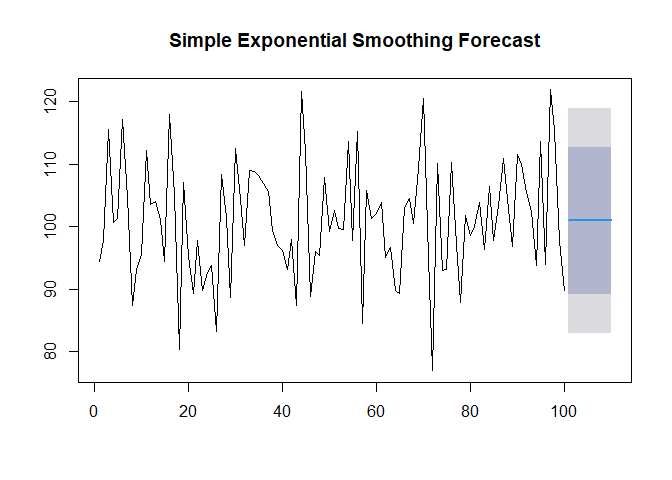
\includegraphics{bassModel_files/figure-latex/unnamed-chunk-3-1.pdf}

\begin{Shaded}
\begin{Highlighting}[]
\CommentTok{\# Compute new adopters at each time step}
\NormalTok{dN\_t }\OtherTok{\textless{}{-}} \FunctionTok{c}\NormalTok{(}\FunctionTok{diff}\NormalTok{(N\_t), }\FunctionTok{tail}\NormalTok{(}\FunctionTok{diff}\NormalTok{(N\_t), }\DecValTok{1}\NormalTok{))  }\CommentTok{\# First derivative (rate of new adoptions)}

\CommentTok{\# Compute contributions of innovators and imitators}
\NormalTok{innovators }\OtherTok{\textless{}{-}}\NormalTok{ p }\SpecialCharTok{*}\NormalTok{ (M }\SpecialCharTok{{-}}\NormalTok{ N\_t)  }\CommentTok{\# p * (Remaining Market)}
\NormalTok{imitators }\OtherTok{\textless{}{-}}\NormalTok{ q }\SpecialCharTok{*}\NormalTok{ (N\_t }\SpecialCharTok{/}\NormalTok{ M) }\SpecialCharTok{*}\NormalTok{ (M }\SpecialCharTok{{-}}\NormalTok{ N\_t)  }\CommentTok{\# q * (Adopters Fraction) * (Remaining Market)}
\NormalTok{new\_adopters }\OtherTok{\textless{}{-}}\NormalTok{ innovators }\SpecialCharTok{+}\NormalTok{ imitators}

\CommentTok{\# Create a data frame for the second plot}
\NormalTok{df2 }\OtherTok{\textless{}{-}} \FunctionTok{data.frame}\NormalTok{(}\AttributeTok{Time =}\NormalTok{ t, }\AttributeTok{New\_Adopters =}\NormalTok{ new\_adopters, }\AttributeTok{Innovators =}\NormalTok{ innovators, }\AttributeTok{Imitators =}\NormalTok{ imitators)}

\CommentTok{\# Plot the adoption components}
\FunctionTok{ggplot}\NormalTok{(df2, }\FunctionTok{aes}\NormalTok{(}\AttributeTok{x =}\NormalTok{ Time)) }\SpecialCharTok{+}
  \FunctionTok{geom\_line}\NormalTok{(}\FunctionTok{aes}\NormalTok{(}\AttributeTok{y =}\NormalTok{ New\_Adopters, }\AttributeTok{color =} \StringTok{"New Adopters"}\NormalTok{), }\AttributeTok{linetype =} \StringTok{"dashed"}\NormalTok{, }\AttributeTok{size =} \FloatTok{1.2}\NormalTok{) }\SpecialCharTok{+}
  \FunctionTok{geom\_line}\NormalTok{(}\FunctionTok{aes}\NormalTok{(}\AttributeTok{y =}\NormalTok{ Innovators, }\AttributeTok{color =} \StringTok{"Innovators"}\NormalTok{), }\AttributeTok{size =} \FloatTok{1.2}\NormalTok{) }\SpecialCharTok{+}
  \FunctionTok{geom\_line}\NormalTok{(}\FunctionTok{aes}\NormalTok{(}\AttributeTok{y =}\NormalTok{ Imitators, }\AttributeTok{color =} \StringTok{"Imitators"}\NormalTok{), }\AttributeTok{size =} \FloatTok{1.2}\NormalTok{) }\SpecialCharTok{+}
  \FunctionTok{scale\_color\_manual}\NormalTok{(}\AttributeTok{values =} \FunctionTok{c}\NormalTok{(}\StringTok{"New Adopters"} \OtherTok{=} \StringTok{"black"}\NormalTok{, }\StringTok{"Innovators"} \OtherTok{=} \StringTok{"red"}\NormalTok{, }\StringTok{"Imitators"} \OtherTok{=} \StringTok{"green"}\NormalTok{)) }\SpecialCharTok{+}
  \FunctionTok{labs}\NormalTok{(}\AttributeTok{title =} \StringTok{"Bass Diffusion Model: Innovators, Imitators, and New Adopters"}\NormalTok{,}
       \AttributeTok{x =} \StringTok{"Time"}\NormalTok{,}
       \AttributeTok{y =} \StringTok{"New Adopters per Time Unit"}\NormalTok{,}
       \AttributeTok{color =} \StringTok{"Legend"}\NormalTok{) }\SpecialCharTok{+}
  \FunctionTok{theme\_minimal}\NormalTok{()}
\end{Highlighting}
\end{Shaded}

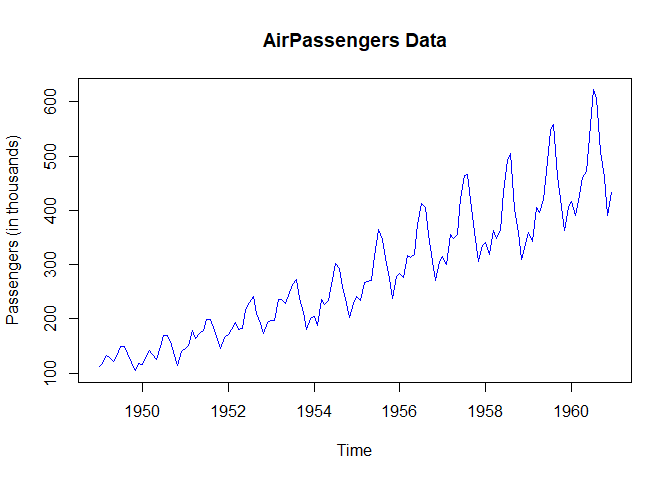
\includegraphics{bassModel_files/figure-latex/unnamed-chunk-4-1.pdf}

\end{document}
